%
%	\section{Plasma sheath}\label{sec:sheathphysics}
%
        \begin{figure}[!b]
			\centering%
			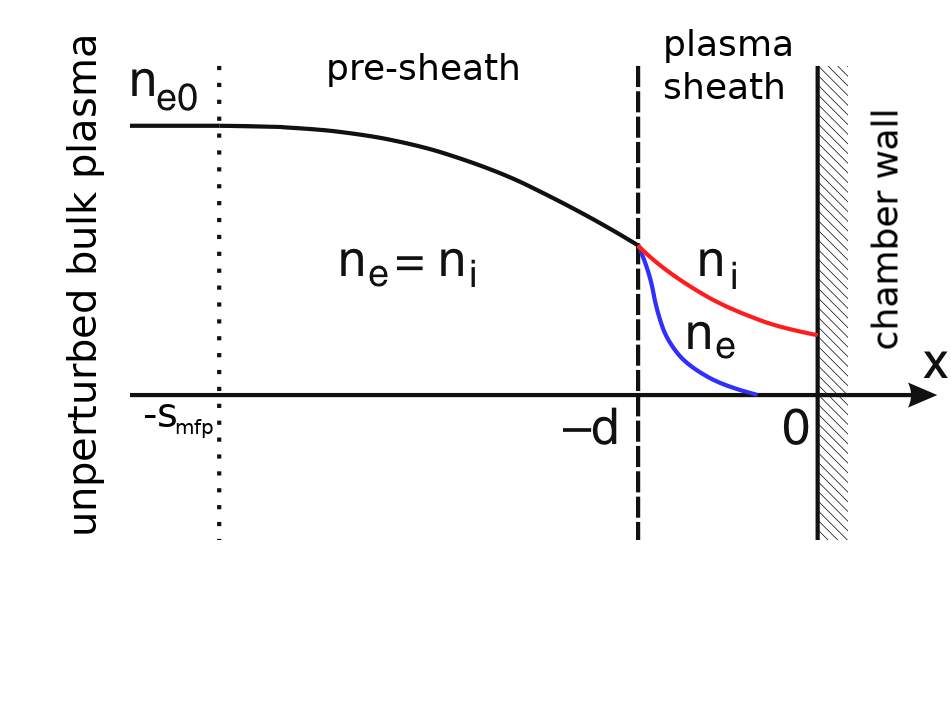
\includegraphics[width=0.8\textwidth]{figures/sheath_piel.png}%
			\caption[1D density profiles as a function of distance and wall potential]{%
    			One dimensional density profiles as a function of the distance to a floating wall. %
    			Note the exponential decrease of the electron density $n\ix{e}$ from the %
    			sheath border towards the negatively charged wall. Densities already reach %
    			approximately 0.66$\cdot n\ix{e,0}$ inside the pre-sheath.~\cite{Piel10}}
			\label{fig:sheath_piel}
		\end{figure}
%
        The electrons are of a much smaller mass in comparison to the other plasma species, which is why they are at least $\sqrt{m\ix{i}/m\ix{e}}$ -- times faster than ions and neutrals. Therefore they have a much higher mobility $\mu\ix{e}$ and thermal velocity $v\ix{th,e}$. For the case of a plasma in front of a surface the larger mobility of electrons lead to an accumulation of a negative charge. To guarantee zero total current to the surface for a steady state, a negative potential drop with respect to the plasma bulk develops in front of the wall to reflect most of the electrons and balance electron and ion currents. A spatially restricted area called \emph{plasma sheath} is established, where the electrons depletion occurs and ions are accelerated towards the wall. The characteristic scale is obviously on the order of some Debye scales, otherwise such a charge separation would not be possible.\\
        The electron density $n\ix{e}(x)$ towards the wall is given by the \emph{Boltzmann} distribution function $f\ix{B}(\Phi)\sim\exp(e\Delta\Phi/k\ix{B}T\ix{e})\,$~\cite{Piel10}. This means that the electron density decreases exponentially towards the negatively charged wall. It can be assumed that the sheath thickness d is much smaller than the mean free path of the ions ($d\ll s\ix{mfp,i}$) inside the plasma bulk. Hence the ions enter the pre-sheath collisionless at a speed $v\ix{i,0}$. The ion and electron densities are therefore:
%
		\begin{align}
			n\ix{i}(x)=n\ix{i}(d){\left(1-\frac{2e\Phi(x)}%
				{m\ix{i}v\ix{i,0}^{2}}\right)}^{-1/2}%
%				\nonumber\\[0.2cm]%
				\quad\text{~and~}\quad
				n\ix{e}=n\ix{e}(d)\exp\left(\frac{e(\Phi(x)-\Phi(d))}{k\ix{B}T\ix{e}}\right)\, .%
				\label{equ:ionandelectrondens}
		\end{align}
%
		One can assume that the kinetic energy of the ions at the sheath entrance is smaller than their potential energy, e.g.\@ $m\ix{i}v\ix{i,0}^{2}\ll |e\Phi(x)|$. Using \emph{Poisson's} equation gives an expression for the potential $\Phi(x)\,$. Solving this, and using the unperturbed ion current $j\ix{i}=n\ix{i}(d)ev\ix{i,0}$, one yields the result by \emph{Langmuir} in~\autoref{equ:langmuirpot}:
%
		\begin{align}
			\Delta\Phi\cong-\frac{en\ix{i}{\left(-d\right)}%
				}{\varepsilon\ix{0}}{\left(-\frac{2e\Phi{%
				\left(x\right)}}{m\ix{i}v\ix{i,0}^2}\right)}^{-\frac{1}{2}}%
			\quad\Rightarrow\quad%
			\Phi{\left(x\right)}=&{\left({\left(\frac{3}{4}{\left(x+d%
				\right)}\right)}^4{\left(\frac{j\ix{i}}{\varepsilon\ix{0}%
				}\right)}^2\frac{m\ix{i}}{2e}\right)}^{\frac{1}{3}}\, .%
				\label{equ:langmuirpot}
		\end{align}
%			
        At $x=-d$, both negative and positive charge density decreased to $n\ix{i}=n\ix{e}\approx\SI{0.66}n\ix{e,0}$ (see~\autoref{fig:sheath_piel}), where the potential is approximately $-k\ix{B}T\ix{e}/2e$.\\
        To satisfy the zero total net current condition $j\ix{e}=j\ix{i}$ the ions are accelerated inside the sheath towards the wall. We know from the above expression for $\Phi(x)$ that the electric field gradient towards the wall is $0<\nabla E<\Delta\Phi$. Using the electron and ion densities one gets the following equation from this: 
%			
			\begin{align} 
				0>&\left.\frac{\diff f}{\diff\Phi}\right|_{\Phi=0}=%
					\frac{en\ix{e}\left(-d\right)}{\varepsilon\ix{0}}\left(\frac{e}%
					{k\ix{b}T\ix{e}}-\frac{e}{m\ix{i}v\ix{i,0}^{2}}\right)%
					\nonumber\\[0.1cm]
                    &\Rightarrow\quad%
					v\ix{i,0}=v\ix{i,B}\ge\sqrt{\frac{k\ix{B}T\ix{e}}{m\ix{i}}}\,,%
					\label{equ:inequality}
			\end{align}
%
            which defines the so-called Bohm criteria for $v\ix{i,B}$ at the sheath edge. One can express this in terms of the \emph{Mach number} $M=v\ix{i,0}/v\ix{i,B}$, where $v\ix{i,B}$ denotes the \emph{Bohm velocity}.\\
            At the sheath edge the quasi-neutrality condition is still satisfied: $n\ix{e}=n\ix{i}\,$. The transport process in the pre-sheath is dominated by collisions with neutral gas particles. Hence the velocity distribution function can be rewritten using the ion-neutral collisions frequency $\nu\ix{n,i}\,$, which becomes
%            
			\begin{align}
				\frac{\diff v\ix{i}}%
				    {\diff x}=\frac{\nu\ix{n,i}v\ix{i}^{2}}%
				    {v\ix{B}^{2}-v\ix{i}^{2}}\quad.%
				\label{equ:distribution}
			\end{align}
%
			From~\autoref{equ:distribution} we can see: ions with velocities smaller than the Bohm velocity are accelerated inside the pre-sheath to Mach equal one or greater according to~\autoref{equ:inequality}:
%
			\begin{align}
				M\ge1%
				\Leftrightarrow%
				v\ix{i}(-d)\ge v\ix{B}\,.%
				\label{equ:bohmcriteria2}
			\end{align}
%
%			\begin{wrapfigure}[16]{r}{0.5\textwidth}
%				\centering%
%				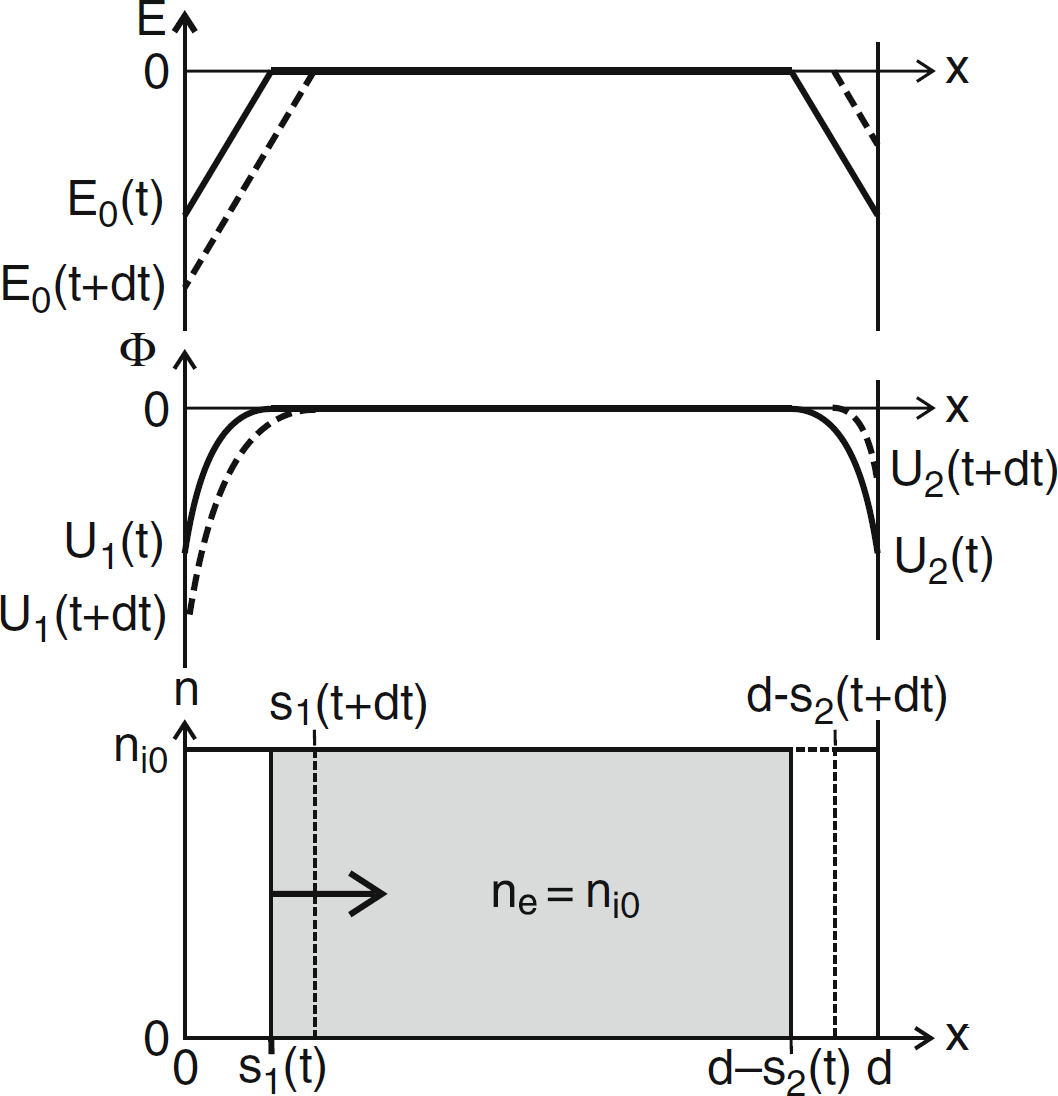
\includegraphics[width=0.45\textwidth]{figures/displacement_current_piel.png}%
%				\caption{%
%					One dimensional density, potential and electric field %
%					for an asymmetric, harmonically driven discharge.%
%					~\cite{Piel10}}\label{fig:displacementcurrent}
%			\end{wrapfigure}
%